\section{Electron-gas models and plasmons}\label{sec:10.3}

Put the Lindhard loss function of the silicon valence electrons into the rate of \cref{sec:10.2}, and a \SI{100}{MeV} particle with a heavy mediator makes $1.31\times10^4$ events per kilogram-year above \SI{1.11}{eV} at $\sigmae = \SI{e-37}{cm^2}$. The crystal tables of \cref{sec:10.2}, with bands, local fields and a gap, give $1.22\times10^4$. A model with one parameter, the electron density, comes within seven percent of the crystal rate. At \SI{1}{MeV} the same model gives 45 times the crystal rate. The gas also carries the plasmon, which at small momentum transfer holds almost the whole $f$-sum, and it is natural to ask whether dark matter can excite it. We derive the electron-gas rate and find where it agrees with silicon and why, then isolate the plasmon pole in the rate and show that halo dark matter falls short of it by about $\omega_p$ in energy and a factor of 3.5 in speed.

\subsection{The Lindhard loss-function rate}\label{sec:10.3-gas}

The electron gas of \cref{sec:4.5} is isotropic, so the direction average in \cref{eq:10.2-rate} does nothing, and its loss function in the random-phase approximation is $\Imag[-1/\varepsilon_{\mathrm{Lin}}(q,\omega)]$ with the Lindhard dielectric function of \cref{eq:4.5-rpa,eq:4.5-lindhard}. Inserting it,
\begin{keyresult}[Electron-gas loss-function rate]
\begin{equation}
  \frac{\dd\mathcal{R}}{\dd\omega} = \frac{\rho_\chi\,\sigmae}{8\pi^2\alpha\,\rho_T\,\mchi\,\mu_{\chi e}^2}\int\dd q\;q^3\,\eta\bigl(\vmin(q,\omega)\bigr)\,\FDM(q)^2\,\Imag\!\left[\frac{-1}{\varepsilon_{\mathrm{Lin}}(q,\omega)}\right] ,
  \label{eq:10.3-gasrate}
\end{equation}
at $T = 0$, with $\varepsilon_{\mathrm{Lin}}$ fixed by the electron density alone through $k_{\mathrm{F}}$ and $\omega_p$. The Mermin form replaces $\varepsilon_{\mathrm{Lin}}$ by $\varepsilon_{\mathrm{Mer}}$ of \cref{eq:4.5-mermin}.
\end{keyresult}
\noindent This is the rate of Knapen, Kozaczuk and Lin with their Lindhard and Mermin functions~\cite[Eqs.~(13), (17) and (19)]{knapen2021dark}. Their prefactor $3\omega_p^2/q^2v_{\mathrm{F}}^2$ is the $k_{\mathrm{TF}}^2/q^2$ of the static Lindhard screening $\varepsilon = 1 + (k_{\mathrm{TF}}^2/q^2)F_{\mathrm{L}}$ (\cref{eq:4.5-static}), since $k_{\mathrm{TF}}^2 = 2e^2\mathcal{N}_{\mathrm{F}} = e^2m_ek_{\mathrm{F}}/\pi^2$ and $\omega_p^2 = e^2k_{\mathrm{F}}^3/3\pi^2m_e$ give $k_{\mathrm{TF}}^2 = 3\omega_p^2/v_{\mathrm{F}}^2$, and their bracket $f^{\mathrm{L}}_1 + \ii f^{\mathrm{L}}_2$ is $-R^0/2\mathcal{N}_{\mathrm{F}}$, the braced expression of \cref{eq:4.5-lindhard}. For silicon the density is that of the four valence electrons per atom, $r_s = 2.0$, $k_{\mathrm{F}} = \SI{3.57}{keV}$ and $\omega_p = \SI{16.6}{eV}$ (\cref{we:4-siplasmon}). Below $q_{\mathrm{c}}$ the gas also has the undamped plasmon of \cref{eq:4.5-plasmonL}, a delta function in $\omega$; we return to it in \cref{sec:10.3-pole} and leave it out of \cref{eq:10.3-gasrate} for now, since halo dark matter cannot reach it.

The comparison with silicon uses the random-phase tables with local fields of \cref{sec:10.2}. Both rates are integrated on the momenta of those tables, from 0.49 to \SI{22.5}{keV}, above the threshold $\Eg = \SI{1.11}{eV}$, the step-model gap that accompanies the tables; their scissor puts the gap at the physical low-temperature value, \SI{1.17}{eV}. Per kilogram-year at $\sigmae = \SI{e-37}{cm^2}$:
\begin{center}
\begin{tabular}{@{}lcccccc@{}}
\toprule
& \multicolumn{2}{c}{\SI{1}{MeV}} & \multicolumn{2}{c}{\SI{10}{MeV}} & \multicolumn{2}{c}{\SI{100}{MeV}} \\
& heavy & light & heavy & light & heavy & light \\
\midrule
Silicon, RPA + LF & 16.7 & 90 & $5.89\times10^4$ & $9.8\times10^3$ & $1.22\times10^4$ & $1.62\times10^3$ \\
Lindhard / silicon & 45 & 70 & 1.42 & 2.6 & 1.07 & 2.1 \\
Mermin / silicon & 54 & 94 & 1.57 & 2.9 & 1.21 & 2.4 \\
\bottomrule
\end{tabular}
\end{center}
The Mermin rows use one term with $\gamma_{\mathrm{rel}} = \SI{3.66}{eV}$, the width of the measured silicon loss peak, which is a fit parameter and not a collision rate (\cref{sec:4.5}).

The gas lacks the gap of silicon and the high-momentum tail of its bound electrons, two errors of opposite sign that set these ratios and that the spectrum of \cref{fig:10-gas-limit} shows. The first is the gap. The gas is a metal. Its continuum reaches down to $\omega = 0$, where $L \simeq e^2m_e^2q\omega/2\pi k_{\mathrm{TF}}^4$ (\cref{sec:4.5}), while silicon has no pairs below its gap and weak absorption up to its peaks at 3.4 and \SI{4.2}{eV} (\cref{fig:4-siloss}). At \SI{100}{MeV} with a heavy mediator the gas spectrum exceeds the crystal one by a factor 24 at \SI{2}{eV} and 4.2 at \SI{3}{eV}. A particle of \SI{1}{MeV} deposits at most $\mchi v_{\mathrm{max}}^2/2 = \SI{3.5}{eV}$ (\cref{eq:1.3-omegamax}), so it samples only this region, and the gas overestimates its rate by a factor 45.

The second error is the momentum distribution of the electrons. The halo deposits at most $\omega = qv_{\mathrm{max}}$ at momentum $q$. In the gas the pairs at $q > 2k_{\mathrm{F}}$ lie in the band $\omega_- < \omega < \omega_+$ around the free recoil $q^2/2m_e$, with $\omega_- = q^2/2m_e - qv_{\mathrm{F}}$, because no electron of the Fermi sea moves faster than $v_{\mathrm{F}}$. The lower edge passes the halo line at $q = 2m_e(v_{\mathrm{F}} + v_{\mathrm{max}}) = \SI{9.85}{keV}$, and beyond it the gas has nothing the halo can reach. The valence electrons of silicon are bound, their orbitals contain momenta above $k_{\mathrm{F}}$, and their loss function keeps weight far below the free recoil. An energy of \SI{20}{eV} needs $q \ge \SI{7.5}{keV}$, and there the gas spectrum is 3 percent of the crystal one; at \SI{15}{eV} it is 27 percent. Between these two regions, from the upper absorption peak at \SI{4.2}{eV} to $k_{\mathrm{F}}v_{\mathrm{max}} = \SI{9.5}{eV}$, the largest energy deposited at $q = k_{\mathrm{F}}$, the valence electrons respond nearly as free electrons do and the gas is within a factor 1.5 of the crystal. That band holds 62 percent of the silicon rate at \SI{100}{MeV}. The integrated agreement at that mass, seven percent, is the excess below the band cancelling the deficit above it. A light mediator weights small $q$ and therefore small $\omega$, where the gas has its excess, and its ratio stays near 2.

The Mermin function does not repair either error. Its relaxation rate spreads the plasmon and gives the loss function a tail $\gamma_{\mathrm{rel}}\omega/\omega_p^2$ below it (\cref{sec:4.5}), which adds 10 to 35 percent to the rates in the table above; the function still has no gap. The Mermin oscillator method of \cref{sec:4.5}, however, does better, because it is a fit. Its terms reproduce the measured optical loss function, gap and absorption peaks included, and each step function removes weight below its onset. The Mermin form only carries the fit to finite $q$, keeping each term's share of the $f$-sum. For silicon the method agrees with the first-principles tables to within 10 percent in the rate above a two-electron threshold, and the uncertainty grows for masses whose rate lies near the gap~\cite[App.~C]{knapen2021dark}. The momentum distribution is still that of a gas, and the two methods differ most at large $\omega$, which carries a small share of the rate above that threshold.

Compared to silicon, the gas is the random-phase approximation for a homogeneous medium; the gap, the local fields and the bound momentum distribution are what the crystal adds. The computed crystal loss function that replaces $\varepsilon_{\mathrm{Lin}}$ is the one of \cref{app:E.6}. The gas needs only $\nd_e$, which follows from the cell volume and the count of valence electrons (\cref{app:A.2}), and it serves as a test of the codes that compute the crystal function (\cref{sec:4.5}).

\begin{limitbox}[Lindhard and Mermin loss-function rates][lim:10.3a]
For a homogeneous electron gas the rate is \cref{eq:10.3-gasrate}, with $\varepsilon_{\mathrm{Lin}}(q,\omega) = 1 + (3\omega_p^2/q^2v_{\mathrm{F}}^2)[f^{\mathrm{L}}_1 + \ii f^{\mathrm{L}}_2]$ and $f^{\mathrm{L}}_1 + \ii f^{\mathrm{L}}_2$ the braced expression of \cref{eq:4.5-lindhard}, or the Mermin function $\varepsilon_{\mathrm{Mer}}$ with a relaxation rate $\gamma_{\mathrm{rel}}$~\cite[Eqs.~(13), (17)--(19)]{knapen2021dark}.
\par\smallskip
{\centering
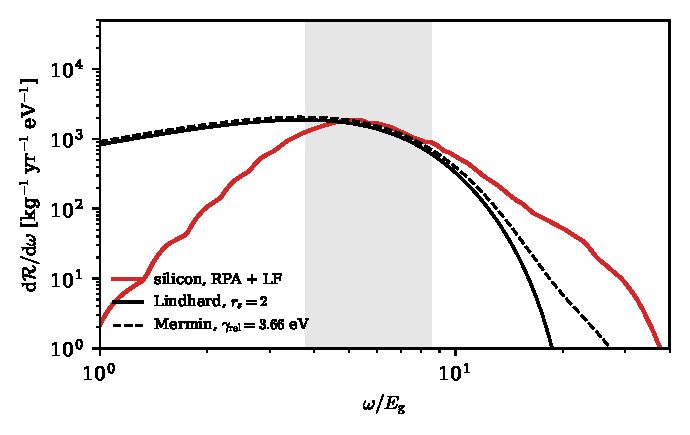
\includegraphics[width=0.82\linewidth]{figures/ch10/limit10_3a.pdf}
\captionof{figure}{Spectrum of silicon at $\mchi = \SI{100}{MeV}$, heavy mediator, $\sigmae = \SI{e-37}{cm^2}$, $\rho_\chi = \SI{0.3}{GeV.cm^{-3}}$ and the standard halo, against $\omega/\Eg$ with $\Eg = \SI{1.11}{eV}$, the step-model gap that accompanies the tables. Red: the random-phase loss function of silicon with local fields (the tables of \cref{fig:10-screening}). Black: the Lindhard loss function of the electron gas at the valence density, $r_s = 2$; dashed, the Mermin function with $\gamma_{\mathrm{rel}} = \SI{3.66}{eV}$, a fit parameter. All three are integrated over the same momenta, from 0.49 to \SI{22.5}{keV}. Gray: from the upper absorption peak of silicon, \SI{4.2}{eV}, to $k_{\mathrm{F}}v_{\mathrm{max}} = \SI{9.5}{eV}$, a band chosen for this figure. There the Lindhard spectrum is between 0.70 and 1.48 times the crystal one.}\label{fig:10-gas-limit}
\par}
\smallskip
Below the band the gas has no gap and overestimates the rate, by 24 at \SI{2}{eV}; above it the gas has no electrons faster than $v_{\mathrm{F}}$ and loses the high-energy tail, and the integrated agreement at this mass comes from the two errors cancelling.
\end{limitbox}

\subsection{Plasmon pole and residue}\label{sec:10.3-pole}

Below $q_{\mathrm{c}}$ the loss function of the gas is the particle--hole continuum plus a line, \cref{eq:4.5-plasmonL}, whose weight is $\pi$ divided by the slope of $\varepsilon_1$ at the zero. At small $q$ the slope follows from the high-frequency expansion of \cref{sec:4.5} kept to order $q^2$~\cite[Eq.~(5)]{kozaczuk2020plasmon},
\begin{equation*}
  \varepsilon_1(q,\omega) \simeq 1 - \frac{\omega_p^2}{\omega^2}\Bigl(1 + \frac{3}{5}\,\frac{q^2v_{\mathrm{F}}^2}{\omega^2}\Bigr) .
\end{equation*}
Its zero is $\omega_{\mathrm{pl}}^2 = \omega_p^2 + \tfrac35q^2v_{\mathrm{F}}^2$, the first two terms of \cref{eq:4.5-dispersion}. With $x = \tfrac35q^2v_{\mathrm{F}}^2/\omega_{\mathrm{pl}}^2$ the zero condition reads $\omega_p^2(1 + x) = \omega_{\mathrm{pl}}^2$, and differentiating,
\begin{gather*}
  \frac{\partial\varepsilon_1}{\partial\omega}\bigg|_{\omega_{\mathrm{pl}}} = \frac{2\omega_p^2}{\omega_{\mathrm{pl}}^3}\,(1 + 2x) = \frac{2}{\omega_{\mathrm{pl}}}\,\frac{1 + 2x}{1 + x} , \\
  \frac{\pi}{\partial\varepsilon_1/\partial\omega} = \frac{\pi\omega_{\mathrm{pl}}}{2}\,Z_L(q) , \qquad Z_L(q) = \frac{1 + x}{1 + 2x} = 1 - \frac35\,\frac{q^2v_{\mathrm{F}}^2}{\omega_p^2} + O(q^4) .
\end{gather*}
The factor $Z_L$ is the residue of the longitudinal photon propagator at the plasmon pole that Kozaczuk and Lin use for the plasmon's polarization vector~\cite[Eq.~(7)]{kozaczuk2020plasmon}; here it is the weight of the line in $L$. The first moment of the line, $\omega_{\mathrm{pl}}\cdot(\pi\omega_{\mathrm{pl}}/2)Z_L = (\pi/2)\omega_p^2(1 + x)(1 - x)$, is the whole $f$-sum to order $q^2$: at small $q$ the plasmon carries all of the oscillator strength, and the continuum none. Integrating \cref{eq:10.2-rate} over the delta function gives
\begin{keyresult}[Plasmon production rate]
\begin{equation}
  \mathcal{R}_{\mathrm{pl}} = \frac{\rho_\chi\,\sigmae}{8\pi^2\alpha\,\rho_T\,\mchi\,\mu_{\chi e}^2}\int_0^{q_{\mathrm{c}}}\dd q\;q^3\,\FDM(q)^2\,\eta\bigl(\vmin(q,\omega_{\mathrm{pl}}(q))\bigr)\,\frac{\pi\omega_{\mathrm{pl}}(q)}{2}\,Z_L(q) ,
  \label{eq:10.3-plrate}
\end{equation}
with $\vmin$ of \cref{eq:1.3-vmin}, the splitting $\Delta_\chi$ included. Beyond the small-$q$ forms, $\omega_{\mathrm{pl}}$ is the exact zero of $\varepsilon_1$ and $(\pi\omega_{\mathrm{pl}}/2)Z_L$ is replaced by $\pi/(\partial\varepsilon_1/\partial\omega)$ there.
\end{keyresult}
\noindent The small-$q$ residue, with $Z_L$ expanded to $1 - \tfrac35q^2v_{\mathrm{F}}^2/\omega_p^2$ as in the limit check below, agrees with the exact one of the Lindhard function to $10^{-4}$ at $q = 0.1\,k_{\mathrm{F}}$ and $8\times10^{-3}$ at $0.3\,k_{\mathrm{F}}$, the size of the dropped $q^4$ terms. Near the cutoff the two part. The exact line carries 0.99 of the $f$-sum at $q_{\mathrm{c}}/2$, 0.77 at $0.9\,q_{\mathrm{c}}$, and nothing at $q_{\mathrm{c}}$. At the continuum edge $\omega_+$ the real part of the Lindhard function contains $(1 - \nu_-^2)\ln|(\nu_- + 1)/(\nu_- - 1)|$ with $\nu_- \to 1$ (\cref{eq:4.5-lindhard}), and its derivative in $\omega$ diverges logarithmically. The slope at the zero therefore grows without bound, and the weight of the line goes to zero as the line touches the continuum. The weight it loses appears in the continuum just below it; this is Landau damping seen in the residue.

The cutoff itself depends on how the dispersion is treated, and the literature uses several values. The exact zero of $\varepsilon_{\mathrm{Lin}}$ meets the edge $\omega_+ = qv_{\mathrm{F}} + q^2/2m_e$ at $q_{\mathrm{c}} = \SI{2.60}{keV}$ and \SI{24.8}{eV} (\cref{sec:4.5}). The quadratic dispersion, with the $q^4$ terms dropped, meets it at \SI{2.24}{keV} and \SI{20.6}{eV}, a dispersion fixed at $\omega_p$ at \SI{1.88}{keV}, and the estimate $\omega_p/v_{\mathrm{F}}$ is \SI{2.38}{keV}. The spread is large because the correction is not small near the cutoff: at \SI{2.24}{keV}, $\tfrac35q^2v_{\mathrm{F}}^2/\omega_p^2 = 0.53$. All four values lie close to the zone scale $2\pi/a = \SI{2.28}{keV}$ of silicon. The crystal shows the same onset (\cref{fig:10-plasmon}). In the silicon tables the loss peak follows the gas dispersion from \SI{18.9}{eV} at \SI{0.5}{keV} to \SI{22.3}{eV} at \SI{2.45}{keV}, with a half-maximum width of about \SI{5}{eV}. Beyond that it broadens fast: at \SI{3.5}{keV} the half maximum spans 17.7 to \SI{32.2}{eV}, and at \SI{4.6}{keV} 14.9 to \SI{44}{eV}. The tables place the small-$q$ peak \SI{2.5}{eV} above the measured \SI{16.4}{eV}, because the scissor that fixes the gap also raises the interband energies that push the plasmon up (\cref{we:4-siplasmon}).

Kurinsky, Baxter, Kahn and Krnjaic wrote the plasmon rate of a fast component of dark matter with a light mediator as the optical line shape times a logarithm~\cite[Eqs.~(13) and (14)]{kurinsky2020dark}. It follows from \cref{eq:10.2-rate} in two steps. A light mediator has $\FDM = (q_0/q)^2$, so $q^3\FDM^2 = q_0^4/q$. Replacing $L(q,\omega)$ by its optical value $L(0,\omega)$ for all $q$ below a cutoff then gives
\begin{equation*}
  \frac{\dd\mathcal{R}}{\dd\omega} = \frac{\rho_\chi\,\sigmae\,q_0^4}{8\pi^2\alpha\,\rho_T\,\mchi\,\mu_{\chi e}^2}\;L(0,\omega)\int_0^{q_{\mathrm{c}}}\frac{\dd q}{q}\;\eta\bigl(\vmin(q,\omega)\bigr) ,
\end{equation*}
which is Ref.~\cite[Eq.~(14)]{kurinsky2020dark} in the book's normalization. They set the cutoff at $2\pi/a \sim \SI{5}{keV}$ with $a$ the lattice spacing~\cite[Eq.~(4)]{kurinsky2020dark}. For silicon, with $a = \SI{5.43}{\angstrom}$, $2\pi/a$ is \SI{2.28}{keV}; \SI{5}{keV} corresponds to a length of \SI{2.5}{\angstrom}, close to the bond length. The error this makes is logarithmic, because the integrand is $1/q$. For a particle of speed $v = 0.1$ the plasmon opens at $q_{\mathrm{min}} = \omega_p/v = \SI{0.17}{keV}$, and moving the cutoff from $q_{\mathrm{c}} = \SI{2.60}{keV}$ to \SI{5}{keV} raises the integral by $\ln(5/0.166)/\ln(2.60/0.166) = 1.24$, or 1.31 from \SI{2.24}{keV}. A measure growing like $q$ would have given $(5/2.60)^2 = 3.7$. The constant optical line shape also ignores the weight the line loses near $q_{\mathrm{c}}$, which removes a further 3 percent of the logarithmic integral. For a fast component the choice of cutoff therefore moves the optical form by 25 to 30 percent, not by a factor of several.

\begin{limitbox}[Plasmon production from the pole of $1/\varepsilon$][lim:10.3b]
Below the cutoff the plasmon is the line $L \simeq (\pi\omega_{\mathrm{pl}}/2)Z_L\,\delta(\omega - \omega_{\mathrm{pl}}(q))$, with $\omega_{\mathrm{pl}}^2 \simeq \omega_p^2 + \tfrac35q^2v_{\mathrm{F}}^2$ and $Z_L \simeq 1 - \tfrac35q^2v_{\mathrm{F}}^2/\omega_p^2$~\cite[Eqs.~(5) and (7)]{kozaczuk2020plasmon}. Kurinsky et al. write the light-mediator rate with $L$ taken at $q = 0$ up to the cutoff~\cite[Eqs.~(4), (13) and (14)]{kurinsky2020dark}.
\par\smallskip
{\centering
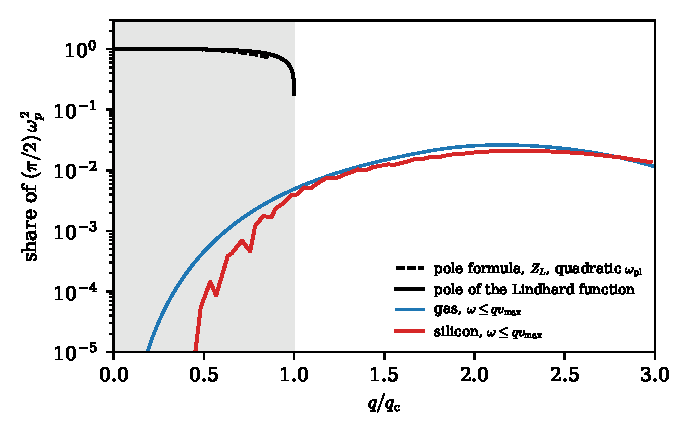
\includegraphics[width=0.82\linewidth]{figures/ch10/limit10_3b.pdf}
\captionof{figure}{Share of the valence $f$-sum $(\pi/2)\omega_p^2$ of silicon, $\omega_p = \SI{16.6}{eV}$, against $q/q_{\mathrm{c}}$ with $q_{\mathrm{c}} = \SI{2.60}{keV}$. Dashed: the first moment of the pole formula, $\omega_{\mathrm{pl}}^2Z_L/\omega_p^2$ with the quadratic dispersion, up to its own cutoff at \SI{2.24}{keV}; dotted: the optical line shape continued to \SI{5}{keV}. Solid black: the pole of the Lindhard function at $r_s = 2$, whose weight falls to zero at $q_{\mathrm{c}}$. Blue: the weight of the Lindhard continuum below $\omega = qv_{\mathrm{max}}$, the most a halo particle can deposit; red: the same for the random-phase loss function of silicon with local fields, from \SI{0.49}{keV}. Gray: $q < q_{\mathrm{c}}$, where the pole exists.}\label{fig:10-pole-limit}
\par}
\smallskip
Near $q_{\mathrm{c}}$ the small-$q$ residue misstates the line, whose weight goes to zero at the continuum edge, and beyond $q_{\mathrm{c}}$ there is no line at all. The weight within reach of the halo is never more than about 3 percent of the $f$-sum and lies in the pair continuum.
\end{limitbox}

\subsection{Plasmon threshold speed}\label{sec:10.3-reach}

A particle of speed $v$ makes a plasmon of momentum $q$ only if $v \ge \vmin(q,\omega_{\mathrm{pl}}(q)) = \omega_{\mathrm{pl}}(q)/q + q/2\mchi$ for elastic scattering, and \cref{eq:10.3-plrate} is nonzero only if this holds for some $q < q_{\mathrm{c}}$. The phase velocity $\omega_{\mathrm{pl}}/q$ is infinite at $q \to 0$ and falls as $q$ grows. At $q_{\mathrm{c}}$ the line meets the continuum edge, where $\omega_{\mathrm{pl}} = \omega_+$ and $\omega_+/q = v_{\mathrm{F}} + q/2m_e$, which rises with $q$; in the Lindhard function the phase velocity reaches its smallest value at $0.989\,q_{\mathrm{c}}$, within $10^{-3}$ of its value at $q_{\mathrm{c}}$. For a heavy particle the slowest one that can make a plasmon therefore moves at
\begin{equation}
  v_{\mathrm{th}} \simeq \frac{\omega_+(q_{\mathrm{c}})}{q_{\mathrm{c}}} = v_{\mathrm{F}} + \frac{q_{\mathrm{c}}}{2m_e} ,
  \label{eq:10.3-vth}
\end{equation}
plus $q_{\mathrm{c}}/2\mchi$ for a finite mass. The threshold is set by the electrons, not by the dark matter. The plasmon is undamped only while its phase velocity exceeds $\omega_+/q$, the largest ratio of energy to momentum that a single pair can have, so the slowest plasmon is as fast as the fastest pair. At the silicon valence density $v_{\mathrm{th}} = 9.54\times10^{-3}$, or \SI{2860}{km.s^{-1}}, and with the quadratic dispersion and its cutoff at \SI{2.24}{keV}, $9.18\times10^{-3}$ or \SI{2750}{km.s^{-1}}. Either is 3.5 to 3.6 times the largest speed of the halo, $v_{\mathrm{max}} = \SI{794.5}{km.s^{-1}}$ (\cref{eq:1.2-vmax}), and agrees with the estimate $v \gtrsim 10^{-2}$ of Kurinsky et al.~\cite[Eq.~(7)]{kurinsky2020dark}. \Cref{we:4-siplasmon} reached the same conclusion from the other side: the line $\omega = qv_{\mathrm{max}}$ reaches $\omega_p$ only at $q = \SI{6.27}{keV}$, more than twice $q_{\mathrm{c}}$.

\begin{figure}[tbp]
  \centering
  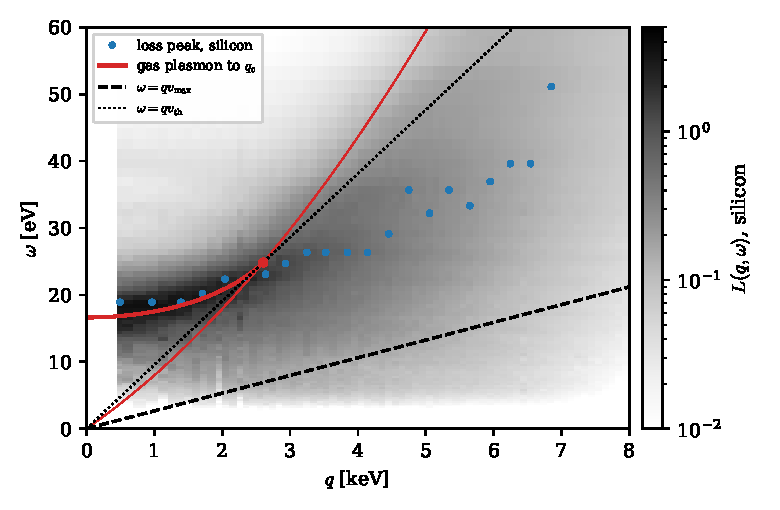
\includegraphics[width=0.9\linewidth]{figures/ch10/fig10_3.pdf}
  \caption{The silicon plasmon against the reach of halo dark matter. Gray scale: the random-phase loss function of silicon with local fields, $L(q,\omega)$, from the tables of Knapen, Kozaczuk and Lin~\cite{knapen2021dark}, averaged over the directions of $\vect{q}$ in bins of \SI{100}{eV} in $|\vect{q}|$ starting at \SI{0.49}{keV}, logarithmic scale. Blue dots: the maximum of $L$ in every third bin. Red: the undamped plasmon of the electron gas at the valence density, the exact zero of $\varepsilon_{\mathrm{Lin}}$, up to $q_{\mathrm{c}} = \SI{2.60}{keV}$ (dot), and the continuum edge $\omega_+ = qv_{\mathrm{F}} + q^2/2m_e$ (thin). Dashed: $\omega = qv_{\mathrm{max}}$, the largest energy a halo particle deposits at momentum $q$. Dotted: $\omega = qv_{\mathrm{th}}$ with $v_{\mathrm{th}} = 9.54\times10^{-3}$ of \cref{eq:10.3-vth}, the slowest particle that reaches the plasmon of the gas. The tables place the small-$q$ loss peak at \SI{18.9}{eV}, against the measured \SI{16.4}{eV}, because of the scissor shift that fixes their gap.}
  \label{fig:10-plasmon}
\end{figure}

In the standard halo the speed distribution ends at $v_{\mathrm{max}}$, and $\mathcal{R}_{\mathrm{pl}}$ is zero at every mass. The suppression is not a power of a small ratio. Remove the escape cut and keep the Maxwellian tail of \cref{sec:1.2}: the fraction of particles faster than \SI{2750}{km.s^{-1}} in the laboratory is about $10^{-49}$, and about $10^{-53}$ above \SI{2860}{km.s^{-1}}. A real halo is not Maxwellian that far out, and these numbers only measure how far the plasmon lies from the bulk of the distribution, 10.5 to 11 times $v_0$ beyond the speed of the Earth.

\begin{workedexample}{The plasmon rate of silicon at the highest halo speed}\label{we:10-plasmon}
Take a particle at $v = v_{\mathrm{max}} = 2.650\times10^{-3}$, heavy enough that $q/2\mchi$ is negligible; at \SI{100}{MeV} it raises $v_{\mathrm{th}}$ by 0.14 percent. At momentum $q$ it deposits at most $qv_{\mathrm{max}}$: \SI{5.94}{eV} at the quadratic cutoff \SI{2.24}{keV}, \SI{6.90}{eV} at $q_{\mathrm{c}} = \SI{2.60}{keV}$. The plasmon of the gas sits at 20.6 and \SI{24.8}{eV} there. The distance between the plasmon and the reach, $\omega_{\mathrm{pl}}(q) - qv_{\mathrm{max}}$, is smallest at $q = \SI{1.34}{keV}$, where it is \SI{14.7}{eV} for the exact zero of the Lindhard function (the quadratic dispersion gives \SI{14.5}{eV} at \SI{1.72}{keV}). The particle is short of the plasmon by about $\omega_p$, at every momentum where the plasmon exists, and \cref{eq:10.3-plrate} gives $\mathcal{R}_{\mathrm{pl}} = 0$.

The silicon plasmon is not a sharp line: interband pairs give it a width of \SI{3.7}{eV} already at $q \to 0$ (\cref{we:4-siplasmon}). The tables show what the particle meets instead. In the bin at \SI{2.28}{keV} the loss peak sits at \SI{22.3}{eV}, and at the reach of the particle, \SI{6.0}{eV}, $L$ is 6.9 percent of its peak value; the energies the particle can deposit hold $1.7\times10^{-3}$ of the valence $f$-sum. At \SI{2.57}{keV} the numbers are 8.5 percent and $4.0\times10^{-3}$. These are pairs on the low-energy side of the resonance, the same pairs that the rate of \cref{sec:10.2} already counts. They also carry little of that rate. At \SI{100}{MeV}, momenta below \SI{2.60}{keV} give $4.9\times10^{-4}$ of the heavy-mediator rate (\num{9.6e-5} below \SI{2.24}{keV}) and 2.5 percent of the light-mediator rate.

The answer is that the plasmon rate of silicon is zero for halo dark matter, not small: the pole needs \SI{2750}{km.s^{-1}} or more, and the halo stops at \SI{794.5}{km.s^{-1}}. A loss-function rate that seems to contain ``plasmon'' events at 15 to \SI{25}{eV} draws them from $q > \SI{5.7}{keV}$, where \cref{fig:10-plasmon} shows only the broad pair continuum.
\end{workedexample}

The pole opens for a fast component of dark matter, for an exothermic splitting, or when a third body takes the momentum, and each case belongs to another section. A fast component, accelerated or boosted, can exceed $v_{\mathrm{th}}$, and \cref{eq:10.3-plrate} applies with its speed distribution in $\eta$ (\cref{sec:10.9}). An exothermic transition lowers $\vmin$ through $\Delta_\chi < 0$ in \cref{eq:1.3-vmin}, and a particle at $v_{\mathrm{max}}$ reaches the line once $|\Delta_\chi| \gtrsim \SI{14.7}{eV}$, the closest approach of the worked example; \cref{sec:17.3} treats such down-scattering into collective modes. When the dark matter scatters off a nucleus, the recoiling ion can emit a plasmon whose momentum is small, as in bremsstrahlung. Kozaczuk and Lin computed this rate in the electron-gas picture and found it four to five orders of magnitude below the elastic nuclear rate for masses from \SI{10}{MeV} to \SI{1}{GeV}~\cite{kozaczuk2020plasmon}; it is a process of the joint electron--lattice response of \cref{chap:12}.

\subsection{Plasmon decay into pairs and phonons}\label{sec:10.3-decay}

With the nuclei clamped, a plasmon of silicon decays into electron--hole pairs and nothing else. At the measured loss peak, \SI{16.4}{eV}, vertical interband transitions are open, $\varepsilon_2 = 0.22$ where $\varepsilon_1$ vanishes, and the width of the loss peak follows from that value (\cref{we:4-siplasmon}). The branching ratio into pairs is one, and \cref{sec:8.7} showed that the screened pair weights of \cref{eq:8.7-screened} already contain the plasmon peak, so that a plasmon is not a separate final state of silicon. Its energy is shared by the pairs, and the step model \cref{eq:1.5-step} turns \SI{16.4}{eV} into five; the cascade that produces them is the subject of \cref{sec:18.1}.

With the lattice free to move, part of the decay goes into pairs plus phonons. By the decomposition theorem \cref{eq:8.6-decomp}, the absorptive part of the response at $(\vect{q},\omega_{\mathrm{pl}})$ splits into a zero-phonon sector $S^0$ and a phonon-dressed sector $S^+$. Since $L = \varepsilon_2/|\varepsilon|^2$ and the factor $|\varepsilon|^2$ is common to both sectors, the phonon branching of the plasmon is
\begin{equation}
  B_{\mathrm{pl}}^+(\vect{q}) = \frac{S^+(\vect{q},\omega_{\mathrm{pl}})}{S^0(\vect{q},\omega_{\mathrm{pl}}) + S^+(\vect{q},\omega_{\mathrm{pl}})} = \frac{\varepsilon_2^+(\vect{q},\omega_{\mathrm{pl}})}{\varepsilon_2(\vect{q},\omega_{\mathrm{pl}})} ,
  \label{eq:10.3-branch}
\end{equation}
the share of phonon-assisted absorption in $\varepsilon_2$ at the plasmon energy. At \SI{16}{eV} direct transitions are allowed. A phonon-assisted transition needs one electron--phonon vertex besides the density vertex, and its amplitude carries the vertex over an energy denominator. With optical-phonon vertices of a few tenths of an eV and denominators of a few eV, \cref{sec:6.5} found the phonon-assisted absorption to be about $10^{-2}$ of the direct one per coupled mode. At the plasmon energy the direct transitions are strong, and the same estimate puts $B_{\mathrm{pl}}^+$ between $10^{-3}$ and $10^{-2}$; it has not been computed. The phonons counted by \cref{eq:10.3-branch} always come with a pair. A decay into phonons alone would have to pass \SI{16}{eV} to modes of at most \SI{64}{meV}, some 260 of them, with no electronic final state, and it is not part of this estimate. Kurinsky et al. needed plasmons that decay mostly into phonons to explain low-energy excess events~\cite{kurinsky2020dark}; the estimate here gives a phonon share of at most a percent.

\Cref{sec:10.4} turns from the number of the electrons to their spin and their current.
